	%------------------第一章---------------------------
	\newpage
	\section{绪论}
    \subsection{超声波接近传感器的研究背景和意义}
    \subsubsection{超声波接近传感器的发展}
    超声波接近传感器是一种能够实现非接触测距的传感器。随着现代工业和科技的快速发展,超声波接近传感器的应用领域也在不断扩大,已经成为自动控制、机器人、无人驾驶等领域中不可或缺的组成部分。其发展经历了三个阶段:第一代采用固定式超声波传感器,第二代采用微机处理技术和数字滤波技术,第三代采用了新型材料和新技术,如MEMS技术、FPGA技术等,提高了系统的测量精度、稳定性和抗干扰能力。在未来,超声波接近传感器将进一步发展,应用领域将更加广泛,并且在系统的设计、制造和使用方面还有许多问题和挑战需要解决和克服。
    \subsubsection{超声波接近传感器国内外研究现状}
    \paragraph{国内研究现状}
    中国的超声波接近传感器研究在过去几十年里得到了快速发展。目前,国内大量高校和研究机构已经开始从事这方面的研究,如清华大学、中国科学院声学研究所、南京大学、哈尔滨工业大学等。在研究领域方面,主要集中在新材料、新结构的超声波传感器、嵌入式系统设计、信号处理与模式识别等方面。
    
    同时,超声波接近传感器在国内工业应用中得到了广泛应用,主要应用于物体距离测量、机器人导航、车辆防撞系统、矿井安全监测等领域。在冶金、石化、化工、航空、航天等行业中,也得到了广泛的应用,取得了显著的经济效益和社会效益。
    \paragraph{国外研究现状}
    超声波接近传感器在国外也得到了广泛的应用和研究。美国、日本、德国等发达国家的企业和研究机构在超声波传感技术方面取得了很多创新性成果。美国的Honeywell、日本的松下、德国的西门子等公司都是超声波传感器领域的龙头企业。此外,德国的Fraunhofer公司也是超声波技术研究的领军机构之一,他们致力于超声波传感器的研究和开发,取得了一系列重要进展。
    
    在超声波接近传感器的应用方面,国外的应用场景更加广泛,包括物体检测、精度测量、人体检测、障碍物检测等领域。例如,日本的松下公司在机器人领域应用超声波传感器实现了机器人的自主导航功能;德国的西门子公司在工业自动化领域采用超声波传感器实现了物体的非接触式测量。这些成功的应用案例表明超声波接近传感器在未来的发展中具有广阔的应用前景。
    
    \subsubsection{超声波接近传感器的研究意义}
    在现代工业和自动化控制中,超声波传感器已经成为了一种重要的非接触式测量和检测手段。传统的超声波传感器由于受到环境干扰和传感器本身精度等问题的限制,其应用场景和测量范围受到一定的限制。因此,需要一种高精度、低功耗、多功能的超声波传感器来满足实际应用需求。\par
    TUSS4470芯片作为一种新型的超声波传感器芯片,具有高精度、低功耗和多种工作模式等特点,可以满足现代工业和自动化控制对于测量、检测、控制和导航等方面的需求。因此,基于TUSS4470芯片的超声波接近传感器的研究成为了一个热门话题,其可以应用于智能家居、无人机、自动驾驶车辆、机器人等领域,具有广阔的应用前景和市场前景。\par
    此外,在传统的超声波驱动控制电路中,一般是采用模拟电路或者单片机来控制。由模拟电路驱动的超声波传感器抗干扰性差,而由单片机驱动的超声波传感器,由于其使用外部中断触发的机制,导致无法精确控制时序逻辑,从而难以达到与超声探头匹配的驱动频率,而超声波传感器的检测精度直接取决于其发出脉冲宽度的精度\upcite{CPLD在超声波传感器驱动控制电路中},当脉冲宽度无法匹配时将使得传感器的精度降低,因此使用CPLD芯片控制产生精确的脉冲宽度对提高传感器的检测精度有着十分重要的意义。\par
    本设计采用型号为EPM240T100C5N的MAX II系列芯片,它是一种高集成度、电可擦除、CMOS宏阵列可编程逻辑器件\upcite{基于STM32和超声波测距的倒车雷达预警系统设计},可以产生ns级别的控制信号\upcite{CPLD芯片介绍},配合TUSS4470超声驱动芯片,可精确控制发送脉冲的次数、频率以及脉冲宽度。同时,CPLD芯片编程采用时序逻辑,发送、接收、检测脉冲信号的时间可进行精确控制,这让超声检测策略可以变得更加丰富合理。
    \subsection{超声波接近传感器的原理}
    \subsubsection{超声波介绍}
      超声波是一种弹性机械波,可以在气体、液体和固体中传播。人们可以听到的声音频率范围是$20Hz\sim20KHz$,超出该范围的声音被称为低频声波或超声波。超声波在相同的传播介质里的传播速度相同,在大气条件下的传播速度约为$340m/s$,相对于电磁波的传播速度$3\times10^8m/s$来说非常慢。超声波的纵向分辨率较高,对色彩及光照度不敏感,对外界光线和电磁场不敏感,受环境因素的影响较小,超声波遇到障碍物反射时,入射角和反射角近似相等,方便用于测量较近目标的距离\upcite{车载可视倒车雷达预警系统的研制}。超声波的传播方向与振动方向一致,是纵向振动的弹性机械波,其波动方程描述方法与电磁波相似,如式\ref{波动方程}所示。

    \begin{equation}
    	A=A(x)cos(\omega t+kx)
    	\label{波动方程}
    \end{equation}
	式中\quad$x$---传播距离;
	\quad$\omega$---频率

	\begin{equation}
		A(x)=A_0 e^{-\alpha x}
		\label{振幅方程}
	\end{equation}
	式中\quad$A(x)$---振幅;\par
		\quad$\alpha$---衰减指数
	\begin{equation}
		\alpha=a f^2
		\label{衰减指数}
	\end{equation}
	式中\quad $a$---介质常数;\par
	   \quad $f$---振动频率\par
    根据式\ref{衰减指数}我们可以得出,当频率越高时,振幅衰减程度越大,传播的距离也就越短。声波在空气介质里传播,因空气分子运动摩擦等原因,能量被吸收损耗。同时,超声波频率的过高会引起较多的副瓣,导致近场区的干涉。但是,超声波频率越高,指向性就越强,这一点有利于距离的测量。权衡指向性及损耗两点,为达到良好的测距效果,在设计超声波测距雷达时,我们选用中心频率为$f=30KHz$的超声波 。
    \subsubsection{超声换能器的结构}
    超声换能器是一种将其它形式的能转换为所需频率的超声能或是将超声能转换为同频率的其他形式的能的装置。在实际应用中,常用的超声换能器主要包括电声型和流体动力型两类。
    电声型超声换能器主要包括压电换能器、磁质伸缩换能器和静电换能器三种。其中,压电换能器是最常用的一种,它利用压电效应将电能转化为机械能或将机械能转化为电能\upcite{车载可视倒车雷达预警系统的研制}。磁质伸缩换能器则是利用磁性材料的磁致伸缩效应实现能量转换,静电换能器则是利用静电场的作用实现能量转换。\par
    流体动力型超声换能器主要包括气体和液体两种类型。其中,气体型是利用气体流动产生的声波进行能量转换,液体型则是利用液体流动产生的声波进行能量转换。这两种传感器在实际应用中具有一定的局限性,主要是在响应频率、灵敏度、稳定性等方面存在一定的问题。
    超声换能器的结构形式是多种多样的,不同的超声换能器名称也不尽相同。在超声检测和诊断中,人们通常将超声传感器称作探头。在工业领域中,采用流体动力型传感器的常常被称为“哨”或“笛”,其结构形式也各异\upcite{车载可视倒车雷达预警系统的研制13}。\par
    压电式超声波换能器是一种电声型传感装置,它利用压电材料的特性将电能转换为机械振动,将机械振动转换为电能。压电式超声波换能器主要由压电晶片、楔块、接头等组成,是超声检测中最常用的一种传感装置,是超声波检测装置的重要组成部分。在医学影像诊断、非破坏性检测、声纳定位等领域中得到广泛应用。
    压电材料是压电式超声波换能器的核心材料,分为晶体和压电陶瓷两类。晶体包括石英、妮酸埋等,而压电陶瓷包括错钦酸铅、钦酸钡等。压电材料的特性是在电场中产生应变,在施加外力时产生方向的电场。当对压电材料加交变电场时,它会产生交变应变,从而产生超声振动。
    压电材料可以用来制成超声传感器\upcite{车载可视倒车雷达预警系统的研制14},常见的压电式超声波换能器包括压电陶瓷压电式超声波换能器和晶体压电式超声波换能器。其中,压电陶瓷压电式超声波换能器的灵敏度高、输出稳定,广泛应用于工业领域;而晶体压电式超声波换能器则常用于医疗领域,如超声心动图、超声诊断等。因此,压电材料的选择和设计方案的优化对超声传感器的性能和应用效果有着至关重要的影响。\par
    超声波传感器的核心是压电晶片,它可以产生逆压电效应和正压电效应。当压电晶片接收到发射电脉冲时,逆压电效应会使晶片振动并发射超声波;而当晶片接收到超声波时,正压电效应会使晶片发生机械变形,并将其转换成相应的电信号。通常采用双压电陶瓷晶片制成超声波换能器,其中一个晶片用于发射超声波,另一个用于接收超声波。当压电陶瓷晶片上加有大小和方向不断变化的交流电压时,会产生压电效应,导致晶片产生机械变形。在压电陶瓷晶片上加有频率为$f$的交流电压,会产生相同频率的机械振动,从而推动空气等媒介,发出超声波。在压电陶瓷晶片上有超声机械波作用时,会产生机械变形,从而转换成与超声机械波相同频率的电信号\upcite{车载可视倒车雷达预警系统的研制15}。这些特性使得超声波传感器可以广泛应用于检测、定位、成像等领域。\par
    \begin{figure}[!h]

    	\begin{minipage}{0.5\textwidth}
    		\centering
    		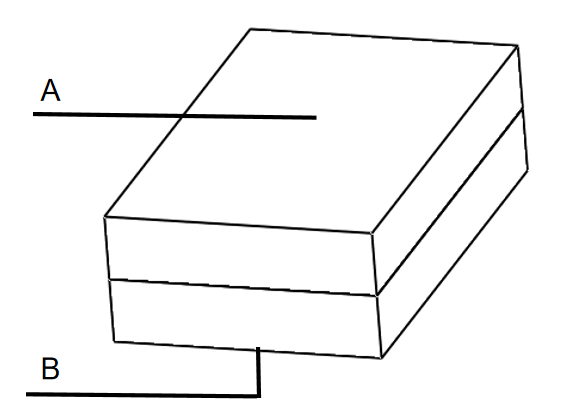
\includegraphics[height=4cm]{figure/双压电晶片示意图.png}
    		\caption{双压电晶片示意图}
    		\label{双压电晶片示意图}
    	\end{minipage}
    \begin{minipage}{0.5\textwidth}
    	\centering
    	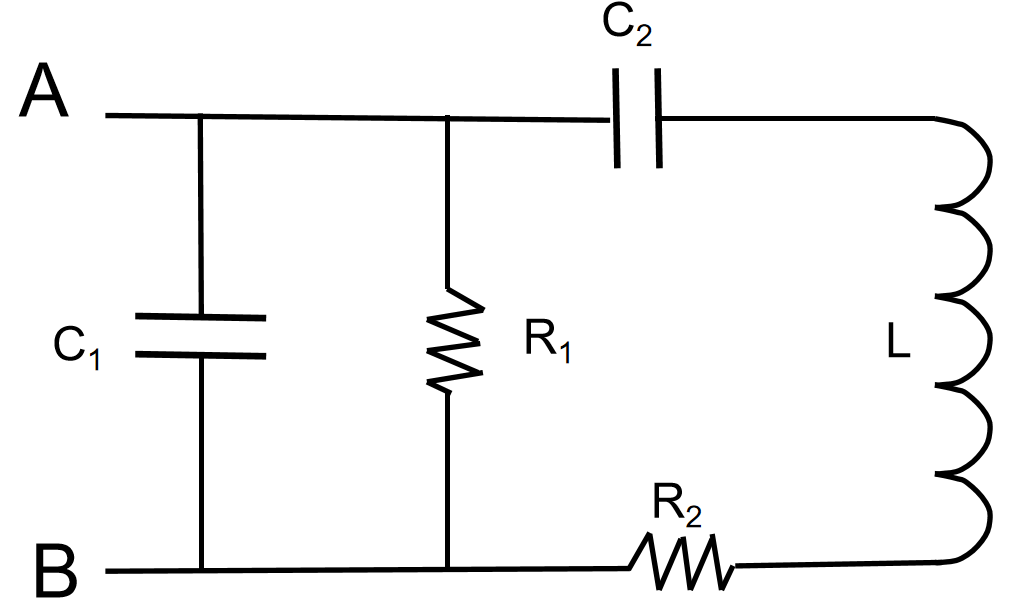
\includegraphics[height=4.25cm]{figure/双压电晶片等效电路.png}
    	\caption{双压电晶片等效电路图}
    	\label{双压电晶片等效电路图}.
    \end{minipage}
    	
 
    \end{figure}
    双压电晶片如图\ref{双压电晶片示意图}所示,当在AB间施加交流电压时,若片的电场方向与极化方向相同,则下面的方向相反,因此,通过上下一伸一缩,形成超声波振动。双压电晶片的等效电路如图\ref{双压电晶片等效电路图}所示。$C_0$为静电电容,$R$为陶瓷材料介 电损耗并联电阻,$C_m$和$L_m$为陶瓷材料介电损耗并联电阻,$R_m$为损耗串联电阻\upcite{51单片机超声波测距仪防撞报警倒车雷达设计}。\par

    压电陶瓷晶片有一个固定的谐振频率,即中心频率$f_0$。发射超声波时,加在其上面的交变电压的频率要与它的固有谐振频率一致。这样超声传感器才有较高的灵敏度。当所用的压电材料不变时,改变压电陶瓷晶片的几何尺寸,就可非常方便的改变其固有谐振频率。利用这一特性就可制成各种频率的超声传感器\upcite{车载可视倒车雷达预警系统的研制16}。
    超声波传感器的结构如图\ref{超声换能器结构图}所示,其主要由金属网、外壳、圆锥形振子、双晶振子、底座和引脚等部分组成 。
    \begin{figure}[!h]
    	\centering
    	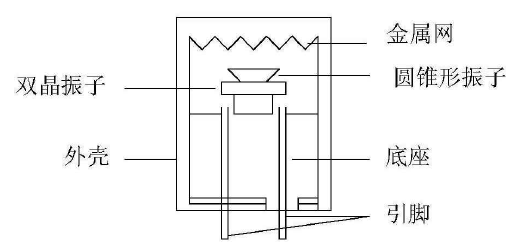
\includegraphics[width=7cm]{figure/超声换能器结构图.png}
    	\caption{超声换能器结构图}
    	\label{超声换能器结构图}
    \end{figure}

    \subsubsection{超声波接近传感器的检测原理}
    \paragraph{连续波相位检测法(CW法))}
    连续波相位检测法的测距原理如图\ref{连续波相位检测法}所示。发射换能器和接收换能器同时发射和接收超声波信号,通过检测信号之间的相位差来获取时间延迟,并计算出传感器与障碍物之间的距离。\par
    \begin{figure}[!h]
    	\centering
    	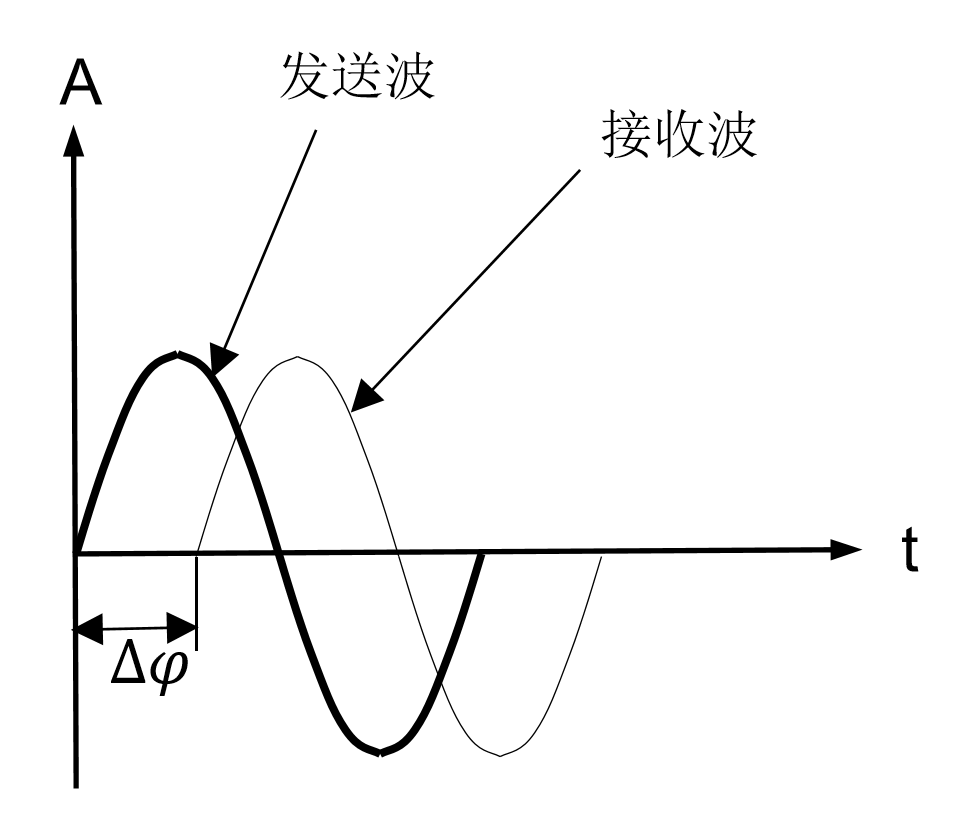
\includegraphics[width=6cm]{figure/连续波相位检测法.png}
    	\caption{连续波相位检测法}
    	\label{连续波相位检测法}
    \end{figure}\par


    假设 发射 的 声 波信 号 为 :
    \begin{equation}
    	u_1=A(x)sin(\omega t + \varphi)
    \end{equation}
式中\quad$\varphi$---初始相位角
接收到的回波信号为:
\begin{equation}
	u_2=A(x)sin(\omega t + \varphi + \omega \cdot{\frac{2D}{c}})
\end{equation}
式中\quad$c$---声速\par
发射声波与回波间的相位差为$\Delta \varphi=\frac{2D}{c}$,传感器与检测物体间的距离D为:
\begin{equation}
	D=\frac{c}{2\omega}\cdot \Delta \varphi=\frac{c}{4\pi f}\cdot(2\pi n + \varphi_i)
\end{equation}
式中\quad$n$---整周期的个数;
\quad$\varphi_i$---不完整周期的相位值。\par
虽然相位检测法的精度比较高,但处理电路的成本也高,需要设计比较复杂的处理电路才能准确地确定回波信号的相位,计算量大\upcite{35}。\par



    
    \paragraph{飞行时间法}
    飞行时间检测法又称脉冲一回波检测法(如图\ref{飞行时间检测法})。超声波发射换能器发射一组超声波脉冲,超声波在遇到障碍物后反射回接收换能器,接收换能器在接收到反射回波时,会与发射时刻之间产生时间延迟,该时间延迟称为超声波的飞行时间$t$,可见飞行时间$t$与声波速度$c$和传播距离$L$有关,即$t=\frac{L}{c}$。\par
    \begin{figure}[!h]
    	\centering
    	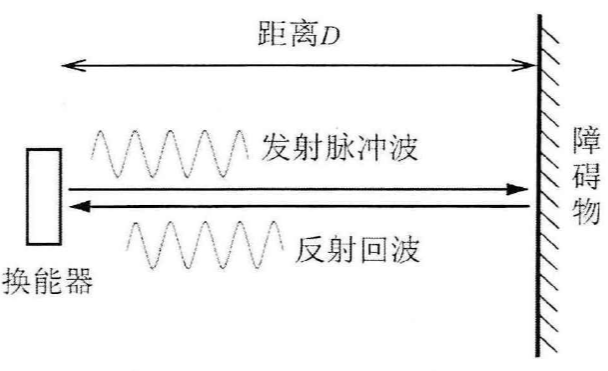
\includegraphics[width=6cm]{figure/飞行时间检测法.png}
    	\caption{飞行时间检测法}
    	\label{飞行时间检测法}
    \end{figure}\par
    飞行时间法最少使用一个换能器便可以实现超声波脉冲的发射和接受,对于自发自收的测距传感器,距离$D$的计算公式为:
    \begin{equation}
    	D=\frac{L}{2}=\frac{ct}{2}
    \end{equation}
	采用飞行时间检测法进行障碍物测距,如何简单准确地获得超声波自发射至接收时的飞行时间,是此方法的关键所在。获取飞行时间的方法有很多种,常见的飞行时间法有:互相关函数法、固定阈值法和包络峰值法。\par
	超声波的回波信号相较于发射信号而言,波形基本不变,但在时间上会有一定延迟,因此这两个信号具有相关性。为了准确获取超声波自发射至接收的飞行时间,可以采用相关函数法进行测量。互相关函数法是对超声波的发射信号和回波信号进行互相关函数计算,函数最大值处所对应的时刻就是收发信号相关性最大的时刻,也是回波信号的接收时刻。通过计算超声波发射时刻与互相关函数最大值时刻之间的时间差,就可以准确获得超声波的飞行时间。除此之外,固定阈值法和包络峰值法也是常用的飞行时间法。\upcite{面向机器人安全避障的MEMS压电超声接近觉传感器的研究}\par
	固定阈值法是指预先设置一个确定的阈值,当接收的回波信号幅值大于此阈值时,认为此信号幅值所在时刻为回波信号的到达时刻,从而获取超声波的飞行时间。但是在回波信号达到预设阈值时,此时所确定的时刻并不是回波信号的起振时刻,具有一定的时间偏差进行时间补偿将其消除后便可获得飞行时间的估计值。阈值预设大小是固定阈值法用于测量距离的关键因素之一。在固定阈值法中,通过将预设阈值与回波信号的幅值进行比较来判断障碍物距离,而阈值的设置会直接影响到测量结果的精确度。如果阈值设置过高,当障碍物距离较远时,回波信号幅值无法达到阈值大小,导致无法获取飞行时间,从而无法准确测量距离。相反,如果阈值设置过低,噪声信号容易达到阈值大小,造成误触发,导致测量结果不可靠。此外,固定阈值法方法还存在其他问题,例如不同反射距离的回波信号波形幅值大小不同,所造成的时间偏差也不同,简单时间补偿无法获得真实飞行时间,进一步降低了测量结果的精确度。因此,虽然固定阈值法方法简单、易实现、计算量不大,但其精度不高,抗干扰能力差的缺点不能忽视。\par
	包络峰值法是一种常见的获取超声波飞行时间的方法。该方法利用回波信号包络线的峰值所在时刻来获取飞行时间。相比于固定阈值法,该方法更加准确,因为回波信号的幅值会随着传播距离的增加而发生变化,而峰值所在的位置相对回波信号的起振时刻并没有发生变化。此外,回波信号的上升时间与超声波发射信号的频率和周期有关,而与传播距离无关,这种特性也使得包络峰值法可以较好地弥补时间偏差,提高测量精度。值得一提的是,包络峰值法同样存在一些缺点,例如受噪声和杂波的影响较大,需要在实际应用中进行适当的干扰抑制和信号处理。\upcite{面向机器人安全避障的MEMS压电超声接近觉传感器的研究38}。
	\paragraph{本设计中的检测原理}
		
    \begin{figure}[!h]
     	\centering
    	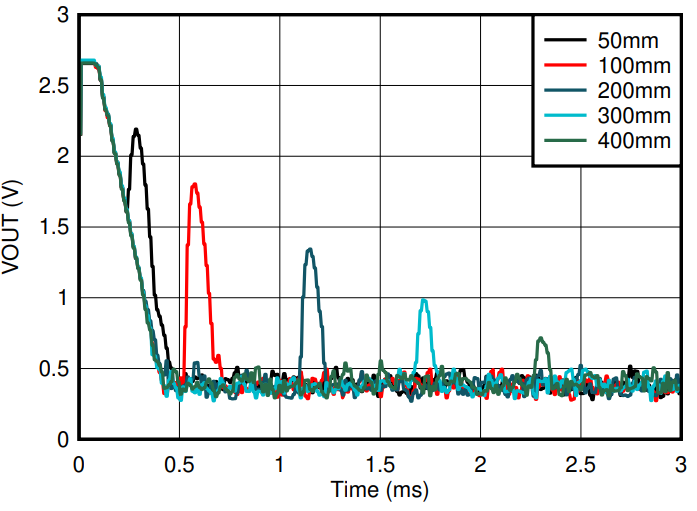
\includegraphics[width=8cm]{figure/VOUT image.png}
    	\caption{VOUT输出}
    	\label{VOUT输出}
    \end{figure}\par
    通过查阅芯片手册\upcite{TUSS4470芯片手册},我们可以知道,TUSS4470芯片采用的检测原理为飞行时间法,获取飞行时间的方法为固定阈值法。\par
    芯片通过滤波解调等处理,可将回波信号处理成一个简单的单峰信号,由VOUT引脚输出,当峰值超过所设定阈值时,即判定为超声换能器接收到回波,该峰值距离起点的时间随检测距离的变化而变化。如图\ref{回波接收模块}所示,当检测物体距离传感器$50mm$、$100mm$、$200mm$、$300mm$、$400mm$时,信号的峰值在不断减小,也在不断地向右侧进行移动。但是在到达有效波峰前,仍然存在着一个波峰信号,影响着物体的检测。通过查阅资料我们得知,这是由于压电振子存在的余振现象所导致的,自发自收的换能器在接收到反射回波时,发射脉冲的余振尚未消失,从而产生一段不能检测回波信号的“盲区”。\par
    波峰距离起点的时间$t$由以下公式得出:       
    \begin{align}
    	t&=t_1+t_2+t_3 \\
    	t&_2=\frac{D}{c}
    	\label{检测周期公式}
    \end{align}  
式中\quad$t$---波峰距离起点时间;\par
    \quad$t_1$---脉冲余振时间;\par
    \quad$t_2$---飞行时间;\par    
    \quad$t_3$---芯片处理回波所花费时间;\par 
    \quad$D$---检测物体距离传感器的距离;\par  
    \quad$c$---声波在空气中的传播速度\par    
    根据任务书中的要求,超声波接近传感器的检测范围为$100mm\sim200mm$,为简化程序,我们通过设定检测窗口的方式来实现该效果。\par  
    当物体与传感器的距离确定时,回波信号波峰对应的$t$也是确定的,该值可以通过实验测得。例如距离为$100mm$、$200mm$时,对应$t$为$1.2ms$、$2.4ms$,那么我们可以设定检测窗口为$1.2ms\sim2.4ms$,只对这个范围内的波峰进行检测,而屏蔽范围外的信号,从而实现不被“盲区”信号所干扰,且检测$100mm\sim200mm$范围物体的功能。\par
    
    
    \subsection{超声波接近传感器研究思路与方法}
    本设计的研究思路和方法涉及多个方面。首先,需要明确设计需求,包括测量范围、测量精度、输出格式等要求,以及硬件和软件的设计要求等。接着,根据设计需求,选择合适的硬件平台。本设计选择了CPLD芯片来控制TUSS4470芯片,以实现测距和数据处理等功能。同时,需要选择合适的电源、滤波电路、放大电路等外围电路,以满足系统的实际应用需求。
    
    在硬件平台确定后,需要编写相应的软件程序,实现数据采集、处理、存储和输出等功能。在软件设计过程中,需要考虑到系统的实时性、准确性和稳定性等要求。基于上述硬件和软件设计,搭建系统原型进行实验测试和验证。根据实验结果调整系统设计,优化算法和参数等。
    
    接着,需要对系统进行进一步的集成和优化,包括系统的可靠性、稳定性、抗干扰性等方面的优化。最后,对系统进行全面的测试和验证,包括系统的性能测试、功能测试、可靠性测试等,以确保系统的稳定性和可靠性。
    
    综上所述,制作基于TUSS4470芯片的超声波接近传感器的研究思路和方法需要综合考虑硬件和软件设计的方方面面,并结合实验测试和验证来不断优化和完善系统设计。